%
% This is the LaTeX template file for lecture notes for EE 382C/EE 361C.
%
% To familiarize yourself with this template, the body contains
% some examples of its use.  Look them over.  Then you can
% run LaTeX on this file.  After you have LaTeXed this file then
% you can look over the result either by printing it out with
% dvips or using xdvi.
%
% This template is based on the template for Prof. Sinclair's CS 270.

\documentclass[twoside]{article}
\usepackage{graphics}
\usepackage{tikz}
\usetikzlibrary{positioning,chains,fit,shapes,calc}

\definecolor{myblue}{RGB}{80,80,160}
\definecolor{mygreen}{RGB}{80,160,80}
\setlength{\oddsidemargin}{0.25 in}
\setlength{\evensidemargin}{-0.25 in}
\setlength{\topmargin}{-0.6 in}
\setlength{\textwidth}{6.5 in}
\setlength{\textheight}{8.5 in}
\setlength{\headsep}{0.75 in}
\setlength{\parindent}{0 in}
\setlength{\parskip}{0.1 in}

%
% The following commands set up the lecnum (lecture number)
% counter and make various numbering schemes work relative
% to the lecture number.
%
\newcounter{lecnum}
\renewcommand{\thepage}{\thelecnum-\arabic{page}}
\renewcommand{\thesection}{\thelecnum.\arabic{section}}
\renewcommand{\theequation}{\thelecnum.\arabic{equation}}
\renewcommand{\thefigure}{\thelecnum.\arabic{figure}}
\renewcommand{\thetable}{\thelecnum.\arabic{table}}

%
% The following macro is used to generate the header.
%
\newcommand{\chapter}[4]{
   \pagestyle{myheadings}
   \thispagestyle{plain}
   \newpage
   \setcounter{lecnum}{#1}
   \setcounter{page}{1}
   \noindent
   \begin{center}
   \framebox{
      \vbox{\vspace{2mm}
    \hbox to 6.28in { {\bf EE 382C/361C: Social Computing
                        \hfill Fall 2018} }
       \vspace{4mm}
       \hbox to 6.28in { {\Large \hfill Chapter #1: #2  \hfill} }
       \vspace{2mm}
       \hbox to 6.28in { {\it Lecturer: #3 \hfill Scribe: #4} }
      \vspace{2mm}}
   }
   \end{center}
   \markboth{Lecture #1: #2}{Lecture #1: #2}
   %{\bf Disclaimer}: {\it These notes have not been subjected to the
   %usual scrutiny reserved for formal publications.  They may be distributed
   %outside this class only with the permission of the Instructor.}
   \vspace*{4mm}
}

%
% Convention for citations is authors' initials followed by the year.
% For example, to cite a paper by Leighton and Maggs you would type
% \cite{LM89}, and to cite a paper by Strassen you would type \cite{S69}.
% (To avoid bibliography problems, for now we redefine the \cite command.)
% Also commands that create a suitable format for the reference list.
\renewcommand{\cite}[1]{[#1]}
\def\beginrefs{\begin{list}%
        {[\arabic{equation}]}{\usecounter{equation}
         \setlength{\leftmargin}{2.0truecm}\setlength{\labelsep}{0.4truecm}%
         \setlength{\labelwidth}{1.6truecm}}}
\def\endrefs{\end{list}}
\def\bibentry#1{\item[\hbox{[#1]}]}

%Use this command for a figure; it puts a figure in wherever you want it.
%usage: \fig{NUMBER}{SPACE-IN-INCHES}{CAPTION}
\newcommand{\fig}[3]{
			\vspace{#2}
			\begin{center}
			Figure \thelecnum.#1:~#3
			\end{center}
	}
% Use these for theorems, lemmas, proofs, etc.
\newtheorem{theorem}{Theorem}[lecnum]
\newtheorem{lemma}[theorem]{Lemma}
\newtheorem{proposition}[theorem]{Proposition}
\newtheorem{claim}[theorem]{Claim}
\newtheorem{corollary}[theorem]{Corollary}
\newtheorem{definition}[theorem]{Definition}
\newenvironment{proof}{{\bf Proof:}}{\hfill\rule{2mm}{2mm}}

% **** IF YOU WANT TO DEFINE ADDITIONAL MACROS FOR YOURSELF, PUT THEM HERE:

\begin{document}
%FILL IN THE RIGHT INFO.
%\chapter{**CHAPTER-NUMBER**}{**DATE**}{**LECTURER**}{**SCRIBE**}
\chapter{10}{Question 13}{Vijay Garg}{Beth Richardson}
%\footnotetext{These notes are partially based on those of Nigel Mansell.}

% **** YOUR NOTES GO HERE:

% Some general latex examples and examples making use of the
% macros follow.  
%**** IN GENERAL, BE BRIEF. LONG SCRIBE NOTES, NO MATTER HOW WELL WRITTEN,
%**** ARE NEVER READ BY ANYBODY.
\section{Question}
Suppose you want to design an auction for the following type of situation: you have two identical copies of a valuable object, and there are four potential buyers for the object. Each potential buyer $i$ wants at most one copy, and has a value $v_i$ for either copy. 

You decide to design the auction by analogy with the way in which we derived the single-item ascending-bid (English) auction from the general procedure for matching markets. In the present case, as there, you want to create a bipartite graph that encodes the situation, and then see what prices the bipartite graph auction procedure comes up with.

\begin{enumerate}
   \begin{enumerate}
   \item Describe how this construction would work using an example with four potential buyers.  In creating your example, first choose specific valuations for the potential buyers, and then show how the auction proceeds and what the market-clearing prices are.
   \item In the case of the single-item auction, the bipartite graph procedure yielded the simple rule from the ascending-bid (English) auction: sell to the highest bidder at the second-highest price. Describe in comparably simple terms what the rule is for the current case of two identical items (i.e. your description should not involve the terms “bipartite”, “graph,” or “matching”
   \end{enumerate}
\end{enumerate}

\section{Answer - a}
We have 2 copies of a valuable object and 4 potential buyers. The following buyers value the object at these valuations:
\begin{center}
 \begin{tabular}{||c c c c||} 
 \hline
 Buyer1 & Buyer2 & Buyer3 & Buyer4 \\ [0.5ex] 
 \hline\hline
 1 & 2 & 3 & 4 \\ 
  \hline\hline
\end{tabular}
\end{center}

\subsection{Auction Begins}
At the beginning of the auction we would have the following bipartite graph:

\begin{tikzpicture}[thick,
  every node/.style={draw,circle},
  fsnode/.style={fill=myblue},
  ssnode/.style={fill=mygreen},
  every fit/.style={ellipse,draw,inner sep=-2pt,text width=2cm},
  ->,shorten >= 3pt,shorten <= 3pt
]

% the buyers
\begin{scope}[start chain=going below,node distance=7mm]
\foreach \i in {1,2}
  \node[fsnode,on chain] (f\i) [label=left: \i] {};
\end{scope}

% the objects
\begin{scope}[xshift=4cm,yshift=-0.5cm,start chain=going below,node distance=7mm]
\foreach \i in {1,2,...,4}
  \node[ssnode,on chain] (s\i) [label=right: \i] {};
\end{scope}

% the set U
\node [myblue,fit=(f1) (f2),label=above:$Objects$] {};
% the set V
\node [mygreen,fit=(s1) (s4),label=above:$Buyers$] {};

% the edges
\draw (f1) -- (s1);
\draw (f1) -- (s2);
\draw (f1) -- (s3);
\draw (f1) -- (s4);
\draw (f2) -- (s1);
\draw (f2) -- (s2);
\draw (f2) -- (s3);
\draw (f2) -- (s4);
\end{tikzpicture}

\subsection{Auction Steps}
In the first step of the auction, both sellers have a price of 0 and all buyers are willing to purchase the items. In the second step of the auction, both sellers have a price of 1 and buyers 2, 3 and 4 are willing to purchase the items. In the third step of the auction, both sellers have a price of 2 and buyers 3 and 4 are both willing to purchase both items. There are no further steps of the auction as both buyers then have purchased items and both items have been purchases.

\subsection{Auction Ends}
At the end of the auction we would have the following bipartite graph, in which Buyer 4 would buy the first copy of the object for the valuation of Buyer 2 (2). Buyer 3 would get the second copy of the object for the valuation of Buyer 2 (2).

\begin{tikzpicture}[thick,
  every node/.style={draw,circle},
  fsnode/.style={fill=myblue},
  ssnode/.style={fill=mygreen},
  every fit/.style={ellipse,draw,inner sep=-2pt,text width=2cm},
  ->,shorten >= 3pt,shorten <= 3pt
]

% the buyers
\begin{scope}[start chain=going below,node distance=7mm]
\foreach \i in {1,2}
  \node[fsnode,on chain] (f\i) [label=left: \i] {};
\end{scope}

% the objects
\begin{scope}[xshift=4cm,yshift=-0.5cm,start chain=going below,node distance=7mm]
\foreach \i in {1,2,...,4}
  \node[ssnode,on chain] (s\i) [label=right: \i] {};
\end{scope}

% the set U
\node [myblue,fit=(f1) (f2),label=above:$Objects$] {};
% the set V
\node [mygreen,fit=(s1) (s4),label=above:$Buyers$] {};

% the edges
\draw (f1) -- (s4);
\draw (f1) -- (s3);
\draw (f2) -- (s4);
\draw (f2) -- (s3);
\end{tikzpicture}


\section{Answer - b}
In this auction, the top and second highest bidder both buy for the valuation of the third highest bidder.


\end{document}





